% 
% PARTIE 2
% 
\section{Étude de la mobilité sur un sol plan \label{sec_2}}


\begin{obj}
L'objectif de cette partie est de valider les performances de mobilité, de manoeuvrabilité et
de contrôle du système de locomotion de ROBOVOLC. On cherche notamment à vérifier le
critère suivant du cahier des charges :

\begin{center}
\begin{tabular}{ll}
\hline
\textbf{Critère} & \textbf{Valeur} \\ \hline 
Vitesse de déplacement atteignable &   \SI{0,5}{m/s} \\\hline
\end{tabular}
\end{center}

\end{obj}



%%%%%%%
%%%%%%%     PARTIE  2.2
%\subsection{Présentation du système de locomotion}
%
%\begin{obj}
%Dans cette sous-partie, on présente l'architecture du système de locomotion de
%ROBOVOLC.
%\end{obj}
%
%
%La plateforme de ROBOVOLC est équipée d'un châssis et de six roues motrices indépendantes et
%non directionnelles réparties symétriquement sur trois essieux (\autoref{fig_04}).
%
%
%\begin{figure}[H]
%\centering
%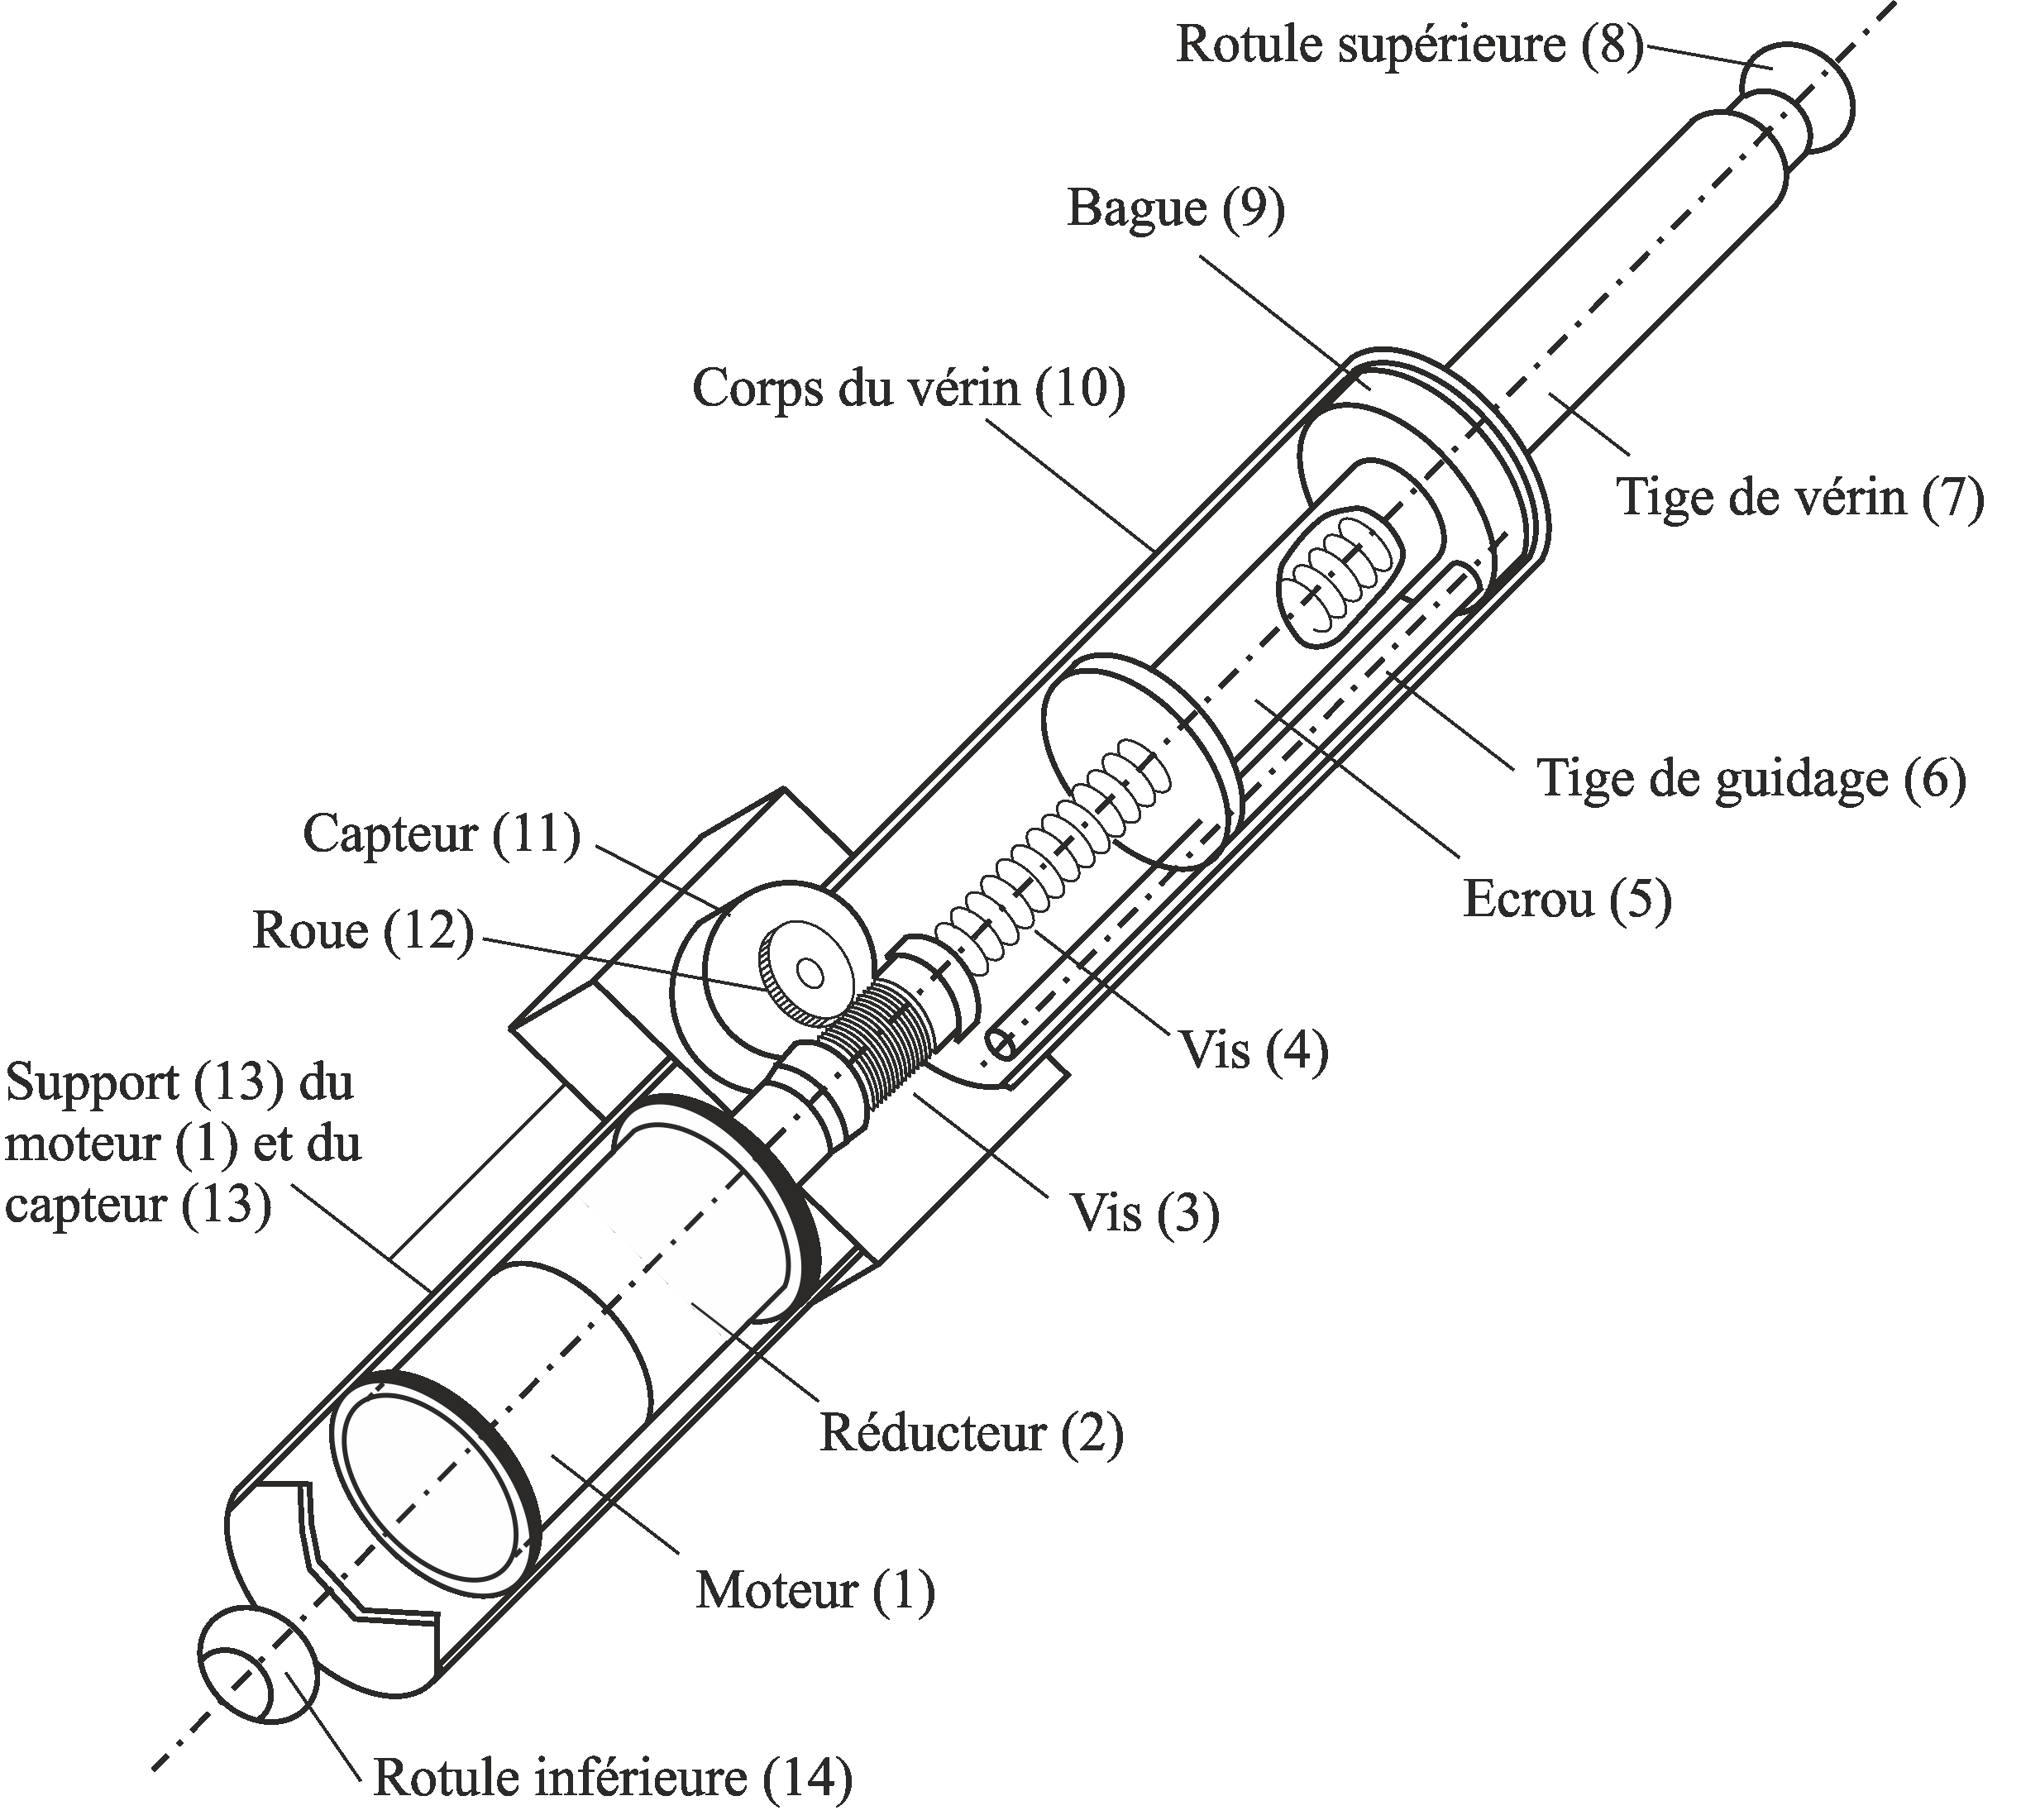
\includegraphics[width=.45\linewidth]{fig_04.png}
%\caption{Schématisation de la plateforme de ROBOVOLC (vue de dessus) \label{fig_04}}
%\end{figure}
%
%
%Chaque roue représente un module autonome (\autoref{fig_05}) dont la chaîne d'énergie est constituée
%d'une batterie, d'un variateur de vitesse, d'un moteur électrique à courant continu, d'un réducteur
%de vitesse (de rapport de réduction $r=\dfrac{1}{236}$, entouré sur la \autoref{fig_05}), d'un capteur de vitesse et
%d'un micro-contrôleur.
%Les roues sont équipées de pneumatiques spéciaux de diamètre extérieur $D=\SI{300}{mm}$.
%
%
%
%\begin{figure}[H]
%\centering
%\includegraphics[width=.45\linewidth]{fig_05w.png}
%\caption{Schéma de transmission de puissance pour chaque roue (vue de dessus) \label{fig_05}}
%\end{figure}
%
%
%On introduit le nombre (adimensionnel) de Froude $Fr=\dfrac{v}{\sqrt{gl_c}}$
%qui caractérise la vitesse de
%déplacement $v$ de ROBOVOLC relativement à sa taille caractéristique $l_c$ ; $g$ est l'accélération de la
%pesanteur. Lorsque $Fr>1$, les effets dynamiques ont une influence importante sur la trajectoire.
%
%%Q2.1 :
%\question{Montrer que les effets dynamiques peuvent être ici négligés.}
%
%Dans la suite de cette partie, on suppose un roulement sans glissement longitudinal au niveau du
%contact roue-sol. On suppose de plus que le sol est plan et horizontal, que le contact roue-sol est
%ponctuel, et que le châssis et les roues sont des solides indéformables.
%
%\subsection{Comportement en ligne droite}
%
%\begin{obj}
%Dans cette sous-partie, on détermine la commande permettant d'assurer une vitesse de
%déplacement en ligne droite donnée.
%\end{obj}
%
%Une modélisation de la plateforme est donnée sur la \autoref{fig_06}. On définit un repère local
%$\repere{O}{x}{y}{z}$ lié au châssis, $\vect{x}$ correspondant à l'axe longitudinal du châssis (appelé aussi ligne de
%foi) illustré sur la \autoref{fig_04}, et $\vect{z} correspondant à l'axe vertical. Le point $O$ est le centre
%géométrique et de masse de la plateforme dans le plan $\left({O},\vect{x}\vect{y}\right)$ parallèle au sol.
%
%Pour chaque roue notée $S_i$ ( $1\leq i \leq 6$), on définit :
%\begin{itemize}
%\item le point de contact $P_i$ entre la roue et le sol ;
%\item le point $O_i$ qui est la projection du point $P_i$ sur l'axe de rotation de la roue.
%\end{itemize}
%
%
%La position de chaque point $O_i$ est définie par $\vect{OO_i}=a_i \vect{x}  +e_i\vect{y}$ avec $a_i=\pm a$ et $e_i=\pm e$.
%Le châssis est noté $S_c$ et le sol est noté $S_0$.

%%%%%%%
%%%%%%%     PARTIE  2.2 PAS FINIE DE RECOPIER !!!!!!



\subsection{Technologie et asservissement en vitesse}
\ifprof\else
Dans cette sous-partie, on étudie l'asservissement en vitesse des roues en analysant la
technologie des composants et en déterminant les propriétés de comportement.
Chacune des roues dispose d'une motorisation indépendante avec un asservissement en vitesse.
Le contrôle de la vitesse de rotation de chaque roue permet de minimiser le glissement
longitudinal, notamment en mode automatique lorsque ROBOVOLC doit suivre un cap de manière
autonome.
Le système d'asservissement qui équipe chaque roue est destiné à contrôler sa vitesse de rotation
et doit permettre au système embarqué de détecter un glissement (manque d'adhérence). Ce
système est modélisé sur la \autoref{fig_07}.

\begin{figure}[H]
\centering
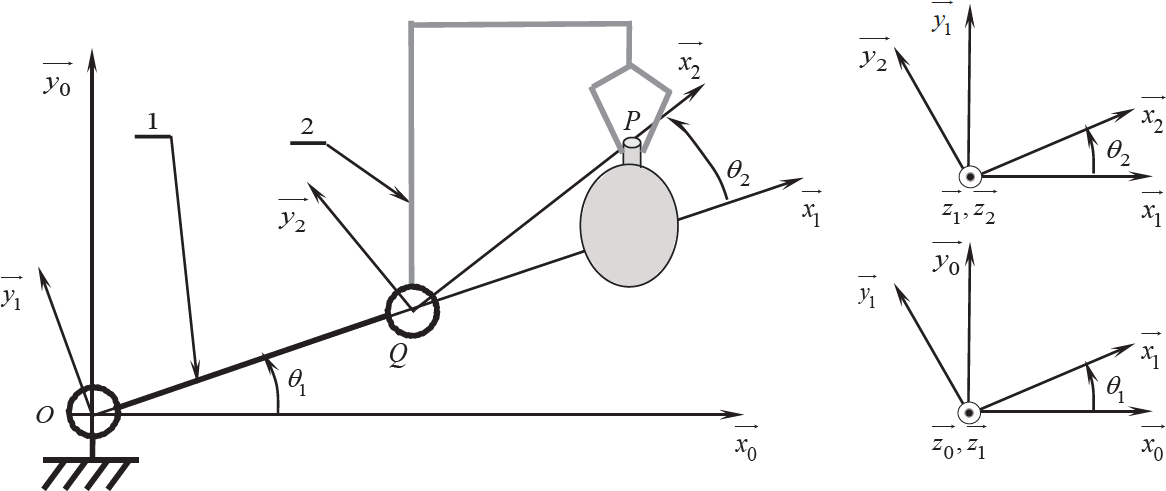
\includegraphics[width=.5\linewidth]{fig_07.png}
\caption{Structure d'asservissement \label{fig_07}}
\end{figure}

La fonction $K_c$ représente un capteur de vitesse permettant de mesurer la vitesse de rotation du
moteur.
\fi


%%Q2.9 :
%\question{Citer deux composants permettant de réaliser la fonction $K_c$ en précisant les
%avantages/inconvénients et le type de signal (analogique ou numérique) en entrée/sortie de
%chacun. Indiquer, en justifiant, la technologie la plus probablement retenue ici.}
%\ifprof
%\begin{corrige}
%\end{corrige}
%\else
%\fi


%Q2.9 :
\question{Citer un composant permettant de réaliser la fonction $K_c$. Décrire succinctement son fonctionnement.}
\ifprof
\begin{corrige}
Une génératrice tachymétrique est un capteur de vitesse. Ce constituant est une machine à courant continu. Lorsqu'il est mis en rotation, il délivre une tension proportionnelle à la vitesse. 
\end{corrige}
\else
\fi

\question{Un codeur incrémental serait-il adapté ? Si oui comment l'utiliser ? Donner la résolution d'un codeur incrémental ayant 1000 fentes et 2 voies de mesures. }
\ifprof
\begin{corrige}
Un codeur est un capteur de position. Connaissant de plus le temps entre deux tops, il est possible de déterminer la vitesse, de l'arbre.

Résolution du codeur incrémental : $\dfrac{360}{1000\times 2 \times 2} = 0,09 \degres$.
\end{corrige}
\else
\fi


\subsubsection{Étude du convertisseur numérique-analogique (CNA)}
\ifprof\else
La valeur $U (t)$ en entrée du CNA est codée sous forme d'un entier non signé sur 16 bits. Elle est
ensuite convertie en grandeur analogique $\indice{U}{mot}$ entre $-\SI{10}{V}$ et $+\SI{10}{V}$ pour $U (t)$ évoluant en hexadécimal de 0000 à sa valeur maximale FFFF.
\fi
%Q2.10 :
\question{Donner la valeur numérique de $U (t)$ à appliquer pour obtenir une valeur nulle en sortie
du CNA. À quelle consigne correspond la valeur hexadécimale d'entrée $U (t) =\text{A000}$?}
\ifprof
\begin{corrige}
On a $U(t) = \left(\text{pts}-2^{15}\right) \times \dfrac{20}{2^{16}}$.
On a $A000 = 10\times 16^3 = 40960 = \SI{2,5}{V}$.  
\end{corrige}
\else
\fi

\subsubsection{Étude du convertisseur analogique-numérique (CAN)}
\ifprof\else
Le capteur utilisé pour mesurer la vitesse de rotation est de type dynamo-tachymétrique, ce choix
répondant aux exigences de tenue en température et robustesse. Le capteur fournit une tension
directement proportionnelle à la vitesse de rotation de la roue, cette tension variant au maximum
entre $-\SI{610}{mV}$ et $+\SI{650}{mV}$. Le CAN employé possède plusieurs canaux de conversion A/N 12 bits
d'une linéarité de $+/-\SI{1}{bit}$. Le temps de conversion par canal est de 25 micro-secondes.
\fi

%Q2.11 :
\question{Calculer la résolution en \si{mV} du CAN.}
\ifprof
\begin{corrige}
On  a : $\dfrac{650+610}{2^{12}} = \SI{0,3}{mV}$.
\end{corrige}
\else
\fi

%Q2.12 :
\question{Dans ces conditions, donner des deux hypothèses principales qu’il faut faire pour pouvoir utiliser un modèle de
système linéaire continu invariant.}
\ifprof
\begin{corrige} \textbf{ -- UPSTI}\\
 Il faut faire l’hypothèse que la période d’échantillonnage soit faible vis-à-vis de la rapidité 
de la grandeur à asservir (pour la validité du modèle système continu). De plus, il faut faire 
l’hypothèse que le pas de quantification est très faible par rapport à l’étendue de mesure de la 
grandeur à asservir (pour la validité du modèle linéaire).
\end{corrige}
\else
\fi

\subsubsection{Asservissement en vitesse}
\ifprof\else
On suppose dans la suite que :
\begin{itemize}
\item $C_v ( p)=K_v$ (constante) ;
\item $K_c =1$ (gain de capteur) ;
\item  les blocs CAN et CNA sont modélisés par des blocs unitaires.
\end{itemize}

La \autoref{fig_08} représente la réponse mesurée du moteur lorsqu’un échelon unitaire de tension est
envoyé en entrée.

\begin{figure}[H]
\centering
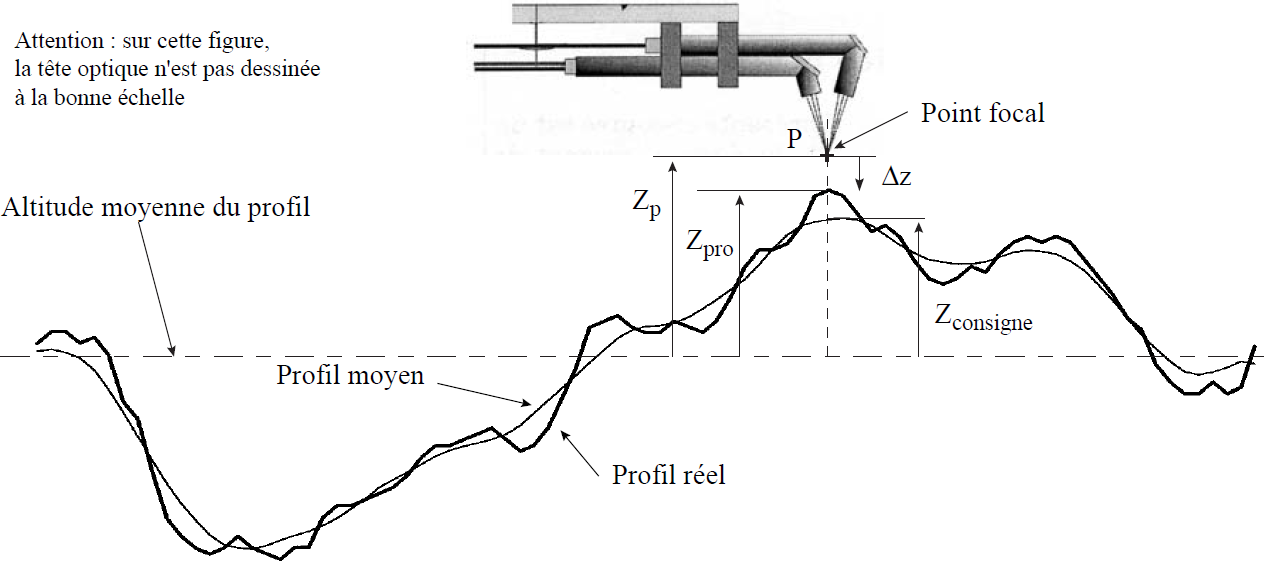
\includegraphics[width=.45\linewidth]{fig_08.png}
\caption{Courbe de réponse du moteur pour un échelon unité\label{fig_08}}
\end{figure}
\fi

%Q2.13 : 
\question{Exprimer par un modèle du premier ordre sous forme canonique la fonction de transfert
$\indice{H}{moteur}( p)$ du moteur, et identifier ses paramètres.}
\ifprof
\begin{corrige}\textbf{ -- UPSTI}\\ 
$H(p)=\dfrac{0,00406}{1+0,34p}$.
\end{corrige}
\else
\fi

Il manque un gain d'adaptation, en amont du comparateur, pour que le système soit asservi sur la vitesse angulaire de la roue.

\question{Déterminer le gain d'adaptation à mettre en amont du comparateur, afin que le système soit asservi sur la vitesse angulaire de la roue.}
\ifprof
\begin{corrige}
Dans ces conditions, l'écart en sortie du premier comparateur doit être nul lorsque l'entrée et la sortie sont égaux. 
On a donc $\varepsilon(p)=\Omega_c(p) \indice{K}{Adapt} -\Omega_m(p) \indice{K}{C} CAN 
=\Omega_c(p) \indice{K}{Adapt} -\dfrac{\Omega_c(p)}{\indice{K}{red}} \indice{K}{C} CAN $.
Il faut donc $\indice{K}{Adapt} = \dfrac{ \indice{K}{C} CAN}{\indice{K}{red}} $

\end{corrige}
\else
\fi

%Q2.14 : 
\question{Calculer la fonction de transfert $\dfrac{\indice{\Omega}{roue}( p)}{\Omega_c(p)}$ sous forme canonique.}
\ifprof
\begin{corrige}
En tenant compte du gain d'adaptation :
$\dfrac{\indice{\Omega}{roue}( p)}{\Omega_c(p)} =\indice{K}{Adapt} \indice{K}{red} \dfrac{C_v(p) CNA \indice{H}{moteur}(p)}{1+C_v(p) CNA \indice{H}{moteur}(p)}$

$=\indice{K}{Adapt} \indice{K}{red} \dfrac{K_v \dfrac{\indice{K}{m}(p)}{1+\tau_m p}}{1+K_v  \dfrac{\indice{K}{m}(p)}{1+\tau_m p}}$
$=\indice{K}{Adapt} \indice{K}{red} \dfrac{K_v \indice{K}{m}}{1+\tau_m p+K_v  \indice{K}{m}}$
$=\dfrac{\indice{K}{Adapt} \indice{K}{red}}{K_vK_m +1} \dfrac{K_v \indice{K}{m}}{1+\dfrac{\tau_m}{K_vK_m +1} p}$

$=\dfrac{\dfrac{ \indice{K}{C} CAN}{\indice{K}{red}} \indice{K}{red}}{K_vK_m +1} \dfrac{K_v \indice{K}{m}}{1+\dfrac{\tau_m}{K_vK_m +1} p}$
$=\dfrac{ \indice{K}{C} CAN }{K_vK_m +1} \dfrac{K_v \indice{K}{m}}{1+\dfrac{\tau_m}{K_vK_m +1} p}$
\end{corrige}
\else
\fi

%Q2.15 : 
\question{Exprimer les conditions pour avoir des valeurs d'erreur statique en position et en vitesse
inférieures à 1\%. Proposer un moyen d'obtenir ces erreurs statiques nulles.}
\ifprof
\begin{corrige}
Le système est de classe 0. Le gain de la BO est donné par $\indice{K}{BO}  = K_v K_m $.
L'écart statique est donc donné par $\varepsilon_S = \dfrac{1}{1+K_v K_m K_c}$. L'erreur de trainage est infinie.
$\varepsilon_S  < 0,01$ si 
$\dfrac{1}{1+K_v K_m} < 0,01$ et donc 
$ \dfrac{1-0,01}{0,01 K_m}<K_v$ soit 
$K_v > 24\,384$.
\end{corrige}
\else
\fi

%% Partie 2.5 TODO
%\subsection{Maîtrise de trajectoire}




